\documentclass[12pt,oneside]{report}
\usepackage[spanish]{babel}
\usepackage[utf8]{inputenc}
\usepackage[T1]{fontenc}
\usepackage{lmodern}
\usepackage{geometry}
\usepackage{setspace}
\usepackage{hyperref}
\usepackage{graphicx}
\usepackage{booktabs}
\usepackage{amsmath,amssymb}
\geometry{margin=2.8cm}
\onehalfspacing

\title{Particion Heterogenea CPU-GPU para Entrenamiento Profundo\\\large Monografia Doctoral (Borrador Evolutivo)}
\author{Doctorando: Zephyr}
\date{\today}

\begin{document}

\maketitle
\tableofcontents
\clearpage

\chapter{Introduccion, Problema y Diseno de la Investigacion}

\section{1.1 Contexto e introduccion}
El entrenamiento de redes neuronales profundas ha incrementado de forma sostenida su complejidad computacional, su densidad paramétrica y sus demandas de memoria, hasta el punto de convertir la disponibilidad de recursos hardware en una condición metodológica del propio resultado científico. En la práctica contemporánea del aprendizaje profundo, la GPU concentra la mayor parte de la carga crítica por su capacidad de cómputo paralelo, mientras que la CPU queda frecuentemente relegada a tareas auxiliares. Sin embargo, esta distribución de funciones no es una ley natural del entrenamiento, sino una convención operativa que responde más a la simplicidad de implementación que a una optimización rigurosa del sistema completo.

La consecuencia inmediata de esa convención es bien conocida: la memoria de la GPU se convierte en el cuello de botella dominante durante el entrenamiento de modelos profundos, especialmente cuando se incrementan resolución, longitud de secuencia, número de capas o tamaño del lote. Al mismo tiempo, la CPU y su espacio de memoria principal permanecen infrautilizados como recurso estructural del proceso de entrenamiento. Esta asimetría no solo limita la escalabilidad, sino que introduce una pregunta de investigación legítima: si la carga del entrenamiento puede distribuirse de forma científicamente controlada entre CPU y GPU, entonces la política de colocación deja de ser un detalle de ingeniería y pasa a constituir un objeto formal de estudio. La literatura sobre rematerializacion, checkpointing y particion automatica confirma que esta tension entre memoria, computo y comunicacion es estructural y no contingente \cite{griewank2000revolve,chen2016sublinear,mirhoseini2017device,jia2019beyond}.

Desde una perspectiva abstracta, el entrenamiento puede entenderse como un proceso de minimización de una función de pérdida sobre un espacio paramétrico:

$$
\theta^* = \arg\min_{\theta} \mathcal{L}(\theta; \mathcal{D}),
$$

pero esa formulación, por sí sola, oculta una dimensión material decisiva: la trayectoria hacia $\theta^*$ depende de una realización física concreta del grafo de entrenamiento. La tesis parte precisamente de esta observación. La optimización estadística del modelo y la organización computacional que la hace posible no son problemas independientes, sino dos caras de un mismo proceso. Por ello, la disponibilidad y la asignación de recursos dejan de ser cuestiones puramente instrumentales y pasan a integrarse dentro del razonamiento científico del trabajo.

La presente monografía se sitúa precisamente en ese punto. Su problema rector no es meramente acelerar código ni describir un conjunto de scripts, sino formular una teoría operacional de la partición heterogénea CPU-GPU para entrenamiento profundo bajo restricciones físicas explícitas. El trabajo entiende la heterogeneidad como un espacio de decisión sobre el cual es posible razonar, medir, optimizar y validar. En consecuencia, la tesis adopta una perspectiva de sistemas y de optimización experimental: mide el comportamiento por capa, robustifica coeficientes, construye un modelo declarativo, transforma la solución en un plan ejecutable y contrasta ese plan con evidencia observada.

Desde esta perspectiva, el valor científico del problema reside en que obliga a unir tres dominios que con frecuencia aparecen separados: la fenomenología empírica del hardware, la formalización matemática de la decisión y la verificación operacional de la política resultante. Si cualquiera de estos planos se omite, el resultado queda metodológicamente incompleto. Una optimización sin datos observados se vuelve abstracta; un profiling sin modelo de decisión es descriptivo pero no normativo; y una solución sin ejecución verificable no alcanza estatuto suficiente de evidencia doctoral en una tesis de sistemas.

En consecuencia, la introducción del problema no puede reducirse a una narrativa de escasez de memoria. Lo que está en juego es la posibilidad de construir una teoría aplicada del entrenamiento heterogéneo donde el diseño del sistema deje de ser un conjunto de decisiones implícitas y se convierta en una política formalmente justificable. Esa transición, desde la intuición ingenieril hacia la decisión explícita bajo restricciones, es el punto de partida conceptual de toda la monografía.

Esta formulacion inicial cumple ademas una funcion de encuadre epistemologico. Permite desplazar el foco desde la pregunta instrumental de si una tecnica concreta acelera o no una corrida hacia una pregunta mas fuerte: bajo que condiciones una redistribucion de computo puede considerarse una decision cientificamente defendible. La diferencia no es retorica. Una mejora puntual de rendimiento puede ser valiosa en ingenieria aplicada; una tesis doctoral, en cambio, debe explicar por que esa mejora es interpretable, reproducible y susceptible de generalizacion conceptual.

En este sentido, la introduccion no opera solo como entrada narrativa al manuscrito, sino como delimitacion del tipo de conocimiento que se busca producir. La tesis no pretende ofrecer una receta local de optimizacion para un modelo particular, sino una forma de pensar la ejecucion heterogenea cuando el hardware deja de ser un soporte transparente y se convierte en parte constitutiva del problema. Esta orientacion es la que justifica el paso desde el analisis descriptivo del entrenamiento hacia una arquitectura metodologica que combina observacion, formalizacion y contraste operacional.

\section{1.2 Motivacion tecnica y relevancia cientifica}
La motivación técnica del trabajo nace de una tensión concreta entre dos hechos empíricos. El primero es que el entrenamiento profundo depende de la retención temporal de activaciones, gradientes y estados del optimizador, lo cual produce una presión acumulativa sobre la memoria de la GPU. El segundo es que la CPU coexiste en la misma plataforma con recursos de memoria y cómputo significativos, pero rara vez participa de manera estructurada en la ejecución del grafo de entrenamiento. La tesis parte de la hipótesis de que esta asimetría no expresa un límite arquitectónico inevitable, sino la ausencia de un marco formal que permita explotar la heterogeneidad sin romper la coherencia operacional del entrenamiento.

Ese marco no puede construirse mediante reubicaciones ad hoc de capas ni mediante intuiciones locales basadas solo en throughput. Requiere una visión integrada de cuatro elementos: costos nodales por capa, dependencias estructurales del grafo, penalización de transferencias entre dispositivos y restricciones de memoria sobre ambos subsistemas. En otras palabras, la CPU no puede incorporarse como recurso complementario útil si la tesis no modela simultáneamente latencia, energía, memoria y comunicación. La dificultad técnica del problema es precisamente que toda decisión local de colocación modifica el equilibrio global del sistema. Ese diagnostico tambien aparece, con diferentes lenguajes, en trabajos sobre paralelizacion de pipeline, particion automatica y optimizacion de colocacion, donde la calidad de la decision depende de dependencias globales y no de reglas locales \cite{huang2019gpipe,narayanan2019pipedream,zheng2022alpa}.

Si se denota de manera esquemática el costo total del entrenamiento como una combinación de cómputo, memoria y comunicación,

$$
Z \sim Z_{comp} + Z_{mem} + Z_{comm},
$$

entonces la motivación técnica del trabajo puede formularse como la búsqueda de políticas que no minimicen un único término de forma miope, sino que controlen el compromiso entre los tres. Un desplazamiento agresivo hacia GPU puede reducir $Z_{comp}$ y, a la vez, volver inviable $Z_{mem}$; un reparto excesivo hacia CPU puede aliviar memoria pero inflar $Z_{comm}$ y degradar el régimen temporal del entrenamiento. La tesis adquiere sentido precisamente porque este compromiso no puede resolverse por intuición local, sino mediante un esquema explícito de decisión.

La relevancia científica surge de convertir ese problema práctico en una metodología reproducible y defendible. La tesis no solo pregunta si la CPU puede participar más, sino bajo qué régimen de restricciones, con qué costo de transferencia, con qué efecto sobre la memoria disponible y con qué consecuencias sobre la calidad final del entrenamiento. En este punto el trabajo se aleja deliberadamente de un enfoque de benchmarking convencional: su meta no es producir una tabla de tiempos, sino un marco de inferencia experimental que permita derivar políticas de asignación interpretables y auditables.

En términos más amplios, el proyecto se inscribe en la transición hacia un aprendizaje profundo consciente de recursos. Esta transición supone que la eficiencia ya no puede definirse exclusivamente por latencia o throughput, sino por la capacidad de sostener entrenamiento útil bajo limitaciones materiales reales. Por ello, la tesis se sitúa en la intersección entre sistemas heterogéneos, optimización discreta y metodología experimental, y adopta como criterio de calidad no la mera novedad algorítmica, sino la coherencia entre medición, modelado y validación.

La relevancia científica del tema reside además en su capacidad de generalización conceptual. Aunque el caso de estudio se desarrolla sobre entrenamiento profundo CPU-GPU, la pregunta subyacente es más amplia: cómo convertir restricciones materiales del sistema en variables explícitas de decisión dentro de un marco formal. En este sentido, la tesis no solo aspira a producir una solución técnica utilizable, sino también a proponer un modo de razonar sobre aprendizaje automático cuando el recurso físico deja de ser abundante y pasa a formar parte del problema mismo.

Esa capacidad de generalizacion es particularmente importante en el contexto contemporaneo del aprendizaje profundo. A medida que los modelos crecen, la distancia entre formulacion estadistica y realizacion material se vuelve mas estrecha. Ya no basta con demostrar que un metodo converge o que una arquitectura mejora una metrica final; es necesario mostrar tambien que tal comportamiento puede sostenerse bajo restricciones realistas de memoria, energia y comunicacion. La motivacion cientifica del trabajo se asienta precisamente en esa mutacion del campo: la eficiencia de sistemas deja de ser un apendice ingenieril y pasa a formar parte del contenido cognitivo de la investigacion.

Por ello, la tesis se coloca deliberadamente en una frontera interdisciplinar. No pertenece unicamente al analisis de sistemas heterogeneos ni exclusivamente al aprendizaje automatico, sino al espacio en que ambos dominios se exigen mutuamente coherencia. Esta posicion hace mas exigente la argumentacion del manuscrito, pero tambien la vuelve mas valiosa: permite que cada resultado pueda leerse a la vez como proposicion sobre entrenamiento profundo y como proposicion sobre organizacion material del computo.

\section{1.3 Planteamiento formal del problema}
El entrenamiento de redes neuronales profundas sigue una secuencia bien definida de operaciones distribuidas entre las fases de propagación hacia adelante (forward) y propagación hacia atrás (backward). Durante el backward, es imprescindible conservar las activaciones intermedias generadas por cada capa, ya que son necesarias para el cálculo de gradientes mediante la regla de la cadena. Este requisito impone una demanda acumulativa y sostenida sobre el subsistema de memoria, particularmente en arquitecturas de redes neuronales que son entrenadas en Unidades de Procesamiento Gráfico (GPU).

En las implementaciones estándar, la totalidad del grafo computacional se asigna a un único dispositivo GPU, bajo la suposición de que su alto rendimiento en paralelo puede compensar las limitaciones físicas de capacidad de memoria. Sin embargo, la memoria disponible en la GPU es fija, jerárquicamente segmentada y no ampliable mediante abstracciones de software. Esta restricción se vuelve crítica al entrenar modelos profundos que procesan entradas de alta resolución o mantienen representaciones internas densas, como en redes tipo Transformers o en canalizaciones convolucionales 3D.

Las técnicas convencionales, incluyendo checkpointing, compresión de tensores, aritmética de baja precisión y rematerialización selectiva, alivian parcialmente la presión sobre la memoria, pero actúan exclusivamente dentro del dominio del acelerador. De forma análoga, los paradigmas de entrenamiento distribuido ofrecen escalabilidad en múltiples nodos GPU, pero no resuelven la saturación de memoria en configuraciones monodispositivo o en entornos con recursos locales limitados.

Por su parte, las Unidades Centrales de Procesamiento (CPU), que coexisten en la misma plataforma física, disponen de capacidades computacionales complementarias, espacios de memoria direccionables más amplios y soporte para ejecución vectorizada. A pesar de estas ventajas, permanecen subutilizadas durante el entrenamiento, no por insuficiencia arquitectónica, sino por la ausencia de un marco formal que permita integrarlas en la asignación de cargas bajo criterios consistentes de rendimiento y viabilidad.

Desde la perspectiva de la optimización discreta, este escenario constituye un problema de asignación por capas en un sistema heterogéneo, donde cada operación debe mapearse a un dispositivo de cómputo sujeto a restricciones observables: capacidad de memoria, latencia de transferencia, coste energético relativo y viabilidad de recomputación de activaciones, streaming o prefetching. El espacio de soluciones debe preservar la semántica de ejecución, respetar las dependencias del grafo y mantener la viabilidad global del sistema.

En consecuencia, la presente investigación aborda la siguiente brecha: la ausencia de un modelo de optimización formalmente definido, resoluble y parametrizado con métricas empíricas, que permita distribuir de forma eficiente las cargas de entrenamiento de los modelos de aprendizaje profundo entre CPU y GPU, minimizando la presión sobre la memoria de los aceleradores y preservando la viabilidad de ejecución, la eficiencia en el entrenamiento y la precisión del modelo en plataformas heterogéneas.

\section{1.4 Hipotesis de investigacion}
El entrenamiento supervisado en redes neuronales profundas implica la ejecución secuencial de operaciones tensoriales a través de múltiples etapas computacionales. Durante la fase de retropropagación, es necesario conservar en memoria las activaciones intermedias para calcular correctamente los gradientes mediante la regla de la cadena. Esta dependencia temporal genera una carga acumulativa sobre el subsistema de memoria de la GPU, cuya capacidad es físicamente limitada, jerárquicamente segmentada y no ampliable mediante software. Tales restricciones condicionan el volumen de activaciones que pueden almacenarse simultáneamente, comprometiendo la viabilidad del entrenamiento en modelos con alta densidad computacional o arquitecturas jerárquicas profundas, donde el almacenamiento intermedio se convierte en un recurso crítico.

En respuesta a este fenómeno, la hipótesis central de esta investigación plantea que es posible reducir la presión sobre la memoria de la GPU durante el entrenamiento de modelos de aprendizaje profundo mediante la distribución estructural de operaciones entre los subsistemas CPU y GPU, formalizada a través de un modelo de optimización discreta por capas, parametrizado con métricas reales de ejecución y aplicable a entornos heterogéneos, sin comprometer la exactitud del modelo ni la viabilidad de ejecución. Esta hipótesis implica que el entrenamiento de modelos de aprendizaje profundo puede reformularse como un problema de asignación computacional con restricciones, basado en recursos físicos medibles y verificables; que técnicas como la rematerialización y la transmisión interdispositivo pueden integrarse como decisiones internas dentro de un marco declarativo de optimización; y que el modelo resultante permite explorar configuraciones de ejecución no triviales, en las que la CPU actúa como un componente activo del grafo computacional, compensando las limitaciones de la GPU mediante la distribución inteligente de operaciones.

La validación de esta hipótesis se llevará a cabo mediante la construcción de un modelo de Programación Lineal Entera (ILP) que formalice la asignación óptima de operaciones, la simulación de su comportamiento sobre grafos de entrenamiento representativos y la comparación experimental de sus resultados frente a esquemas tradicionales centrados en GPU, evaluando indicadores como el uso máximo y promedio de memoria, la penalización en tiempo de ejecución, el consumo energético y la exactitud final del entrenamiento.

\section{1.5 Objetivos general y especificos}
El objetivo general de esta investigación es formular, implementar y validar empíricamente una estrategia estructurada de paralelización para el entrenamiento de redes neuronales profundas, que permita la distribución a nivel de capa de las cargas computacionales entre subsistemas CPU y GPU con el fin de reducir la presión sobre la memoria de los aceleradores y, simultáneamente, preservar la precisión del modelo, la viabilidad de ejecución y la eficiencia energética, bajo restricciones arquitectónicas realistas y métricas de rendimiento observables, aportando un marco metodológico reproducible para el análisis y la optimización del entrenamiento sobre entornos de cómputo heterogéneo.

Los objetivos específicos son los siguientes.

\begin{enumerate}
\item Caracterizar empíricamente el uso de memoria y el comportamiento de ejecución de arquitecturas de redes profundas representativas, identificando factores arquitectónicos y operativos que contribuyen a la saturación de la memoria de la GPU, mediante perfiles obtenidos en entornos reales de CPU y GPU.
\item Formalizar la asignación computacional por capas como un modelo de optimización discreta, incorporando variables de decisión para la colocación en los dispositivos, la persistencia de activaciones, las transferencias entre dispositivos y las estrategias de gestión de memoria, como la rematerialización, el streaming asíncrono y, cuando aplique, el prefetching, sujetas a restricciones de recursos y dependencias del grafo.
\item Parametrizar el modelo de optimización utilizando métricas observadas empíricamente, tales como huella de memoria por capa, latencia de ejecución, consumo energético y limitaciones específicas de cada dispositivo, garantizando que la formulación refleje dinámicas reales de entrenamiento.
\item Evaluar escenarios de ejecución híbrida CPU-GPU aplicando el modelo ILP a grafos de entrenamiento representativos, analizando el impacto de las decisiones de ubicación y recomputación sobre el uso de la memoria, el rendimiento temporal y la eficiencia de la asignación para el ajuste del modelo.
\item Validar experimentalmente el marco propuesto cuantificando el ahorro de memoria, las métricas de rendimiento, la eficiencia energética y la precisión final del modelo, e identificando las condiciones prácticas bajo las cuales la participación de la CPU mejora la eficiencia del entrenamiento frente a estrategias tradicionales centradas en la GPU.
\end{enumerate}

\section{1.6 Alcance decisional fijado (resultado de Fase 0)}
El alcance decisional del trabajo fue fijado explícitamente para evitar una deriva reduccionista de la contribución. La tesis no se compromete con una simple asignación estática única por capa, sino con una formulación fuerte que contempla asignación independiente para \textit{forward} y \textit{backward}, persistencia de activaciones como variable explícita del modelo y compatibilidad con estrategias de transferencia asíncrona y \textit{prefetching}. Esta decisión de alcance es metodológicamente importante porque impide confundir un prototipo parcial con la versión científica comprometida por la investigación.

La consecuencia epistemológica de este cierre es directa. El manuscrito puede utilizar formulaciones base y casos piloto como escalones explicativos, pero no puede presentar esas versiones intermedias como si agotaran la propuesta doctoral. Todo el texto debe leerse a la luz del contrato fuerte: la tesis aspira a una política de partición que no solo elija dispositivo por nodo, sino que gobierne también aspectos de disponibilidad de activaciones y sincronización entre subsistemas.

Desde esta perspectiva, el alcance no es un apartado administrativo, sino un mecanismo de disciplina científica. Fijar lo que la tesis realmente promete evita inflar aportes, ordena la validación por fases y mantiene coherencia entre escritura, software y evidencia. Esta coherencia es especialmente necesaria en un proyecto donde la complejidad técnica podría inducir a presentar como cierre doctoral lo que en realidad sería solo una capacidad exploratoria aún no sometida a contraste suficiente.

\section{1.7 Metodologia general y validacion}
La investigación se desarrolla a partir de un enfoque mixto que combina modelado formal y validación experimental, orientado a optimizar el entrenamiento de redes neuronales profundas bajo restricciones arquitectónicas verificables. El problema se formula de manera declarativa, representando las operaciones del grafo de entrenamiento como entidades discretas asignadas a CPU o GPU, sujetas a limitaciones de memoria, latencia, consumo energético y viabilidad estructural. Cada etapa metodológica se concibe como una instancia formalizable y verificable, sustentada en un modelo computacional explícito, mecanismos de trazabilidad algorítmica y criterios de validación reproducibles, garantizando consistencia y rigor científico.

El marco metodológico se estructura en cinco fases secuenciales e interdependientes. En la primera fase, se caracteriza empíricamente el comportamiento de cargas de trabajo de varios modelos de deep learning en plataformas físicas con CPU y GPU, identificando factores arquitectónicos y operativos que inciden en la saturación de memoria de la GPU. Para ello, se seleccionan arquitecturas representativas por su complejidad secuencial, densidad computacional y sensibilidad a la gestión de activaciones. Las ejecuciones reales se instrumentan con herramientas de perfilado y las métricas obtenidas, uso activo de memoria, duración de cómputo, tamaño de activaciones, latencias de transferencia, consumo energético y limitaciones específicas, se organizan en vectores temporales y matrices de observabilidad que constituyen la base parametrizable del modelo.

En la segunda fase, se formaliza un modelo declarativo sobre el grafo acíclico dirigido que describe el entrenamiento supervisado, donde cada nodo representa una operación diferenciable y las aristas codifican dependencias topológicas. El modelo se formula como un sistema de Programación Lineal Entera con variables binarias que definen la asignación de operaciones a CPU o GPU, la retención o recomputación de activaciones y el uso opcional de técnicas asíncronas como streaming interdispositivo, rematerialización o prefetching. Las restricciones incluyen límites de memoria por dispositivo, preservación del orden de ejecución, penalizaciones energéticas, latencias de transferencia y condiciones necesarias para el aprendizaje supervisado basado en gradientes.

La tercera fase consiste en parametrizar el modelo con las métricas reales obtenidas en la caracterización inicial, asegurando coherencia semántica entre observación y simulación, y minimizando divergencias entre ambos entornos. Se incluyen métricas de huella de memoria por capa, latencia de ejecución, consumo energético y limitaciones específicas. Este conjunto se complementa con un análisis de sensibilidad que varía sistemáticamente parámetros clave, penalizaciones por recomputación, latencia de transferencia y umbrales de memoria, para evaluar la estabilidad estructural de las soluciones y su capacidad de generalización.

Con el modelo parametrizado, en la cuarta fase se resuelven instancias mediante solvers ILP, derivando planes de ejecución que integran asignaciones CPU-GPU y políticas de gestión de memoria. A partir de cada solución, se implementa un simulador que reconstruye la secuencia de operaciones, verificando compatibilidad topológica, factibilidad técnica y cumplimiento de restricciones. El simulador estima el comportamiento agregado en términos de uso de recursos, penalizaciones temporales, solapamiento cómputo-comunicación y eficiencia de asignación. Estos resultados se validan de forma cruzada con ejecuciones físicas preliminares, ajustando discrepancias y comparando las estrategias híbridas con esquemas monolíticos centrados en GPU.

Finalmente, la quinta fase aborda la validación experimental en plataforma física, implementando las soluciones óptimas en PyTorch con asignación explícita de capas a CPU o GPU. Se miden uso activo de memoria, penalizaciones temporales, consumo energético estimado mediante telemetría interna y precisión final del modelo. Esta validación confirma tanto el rendimiento técnico como la coherencia metodológica del modelo, contrastando los resultados con esquemas tradicionales y verificando la solidez de sus supuestos en entornos heterogéneos reales.

En conjunto, este flujo metodológico integral y reproducible asegura que las decisiones de asignación optimizadas mantengan su viabilidad tanto en simulación controlada como en ejecución práctica, demostrando eficiencia operativa y consistencia de resultados bajo condiciones reales de cómputo heterogéneo.

\section{1.8 Contribucion cientifica}
La contribución científica de esta investigación radica en la formalización, validación empírica y aplicación de un modelo declarativo de optimización a nivel de capa para el entrenamiento de redes neuronales profundas en entornos heterogéneos CPU-GPU. Este modelo reinterpreta el entrenamiento supervisado como un problema estructurado de asignación, en el que las operaciones computacionales se redistribuyen de manera consistente, verificable y eficiente entre CPU y GPU, respetando las restricciones arquitectónicas observadas en plataformas reales.

A diferencia de los esquemas tradicionales centrados en la GPU, el enfoque propuesto busca reducir la presión de memoria activa sobre el acelerador mediante decisiones explícitas de rematerialización, desplazamiento computacional y sincronización entre dispositivos, preservando la exactitud del modelo y la viabilidad operativa. El sistema formal, basado en Programación Lineal Entera sobre grafos acíclicos de cómputo, integra métricas reales de ejecución tanto en la función objetivo como en las restricciones, garantizando que las soluciones generadas reflejen un comportamiento medible bajo condiciones reproducibles.

Metodológicamente, la investigación se apoya en la secuencia estructurada en la sección de metodología. Este proceso abarca la observación empírica, el modelado computacional, la resolución algorítmica, la simulación híbrida y la validación experimental. El flujo de trabajo está diseñado para ser replicable en distintos contextos arquitectónicos, diseños reales de redes neuronales y marcos de entrenamiento, y es extensible a sistemas multi-GPU, esquemas de memoria distribuida y arquitecturas heterogéneas emergentes con soporte para ejecución asíncrona en CPU.

Asimismo, el estudio introduce la noción operativa de sensibilidad arquitectónica, que evalúa la estabilidad de las soluciones óptimas frente a variaciones controladas en parámetros críticos, como latencia, penalizaciones energéticas y capacidad de retención de memoria. Este análisis no solo facilita la selección de configuraciones optimizadas, sino que también aporta información valiosa sobre el espacio de diseño técnico de los sistemas heterogéneos.

En consecuencia, la tesis presenta un marco computacional formalmente fundamentado y validado empíricamente para el entrenamiento de redes neuronales profundas con conciencia de recursos. Este marco permite razonar de forma sistemática sobre los compromisos entre memoria y rendimiento, apoya el desarrollo de estrategias de ejecución energéticamente eficientes y contribuye al rediseño de flujos de entrenamiento en entornos con saturación de GPU.

La originalidad de esta propuesta radica en integrar un modelo declarativo formal con métricas empíricas de ejecución para guiar la asignación óptima de operaciones en entornos heterogéneos. Su impacto potencial se extiende más allá del caso de estudio, ofreciendo a la comunidad de HPC y Deep Learning una herramienta metodológica replicable, adaptable a nuevas arquitecturas y capaz de influir en el diseño futuro de sistemas y algoritmos de entrenamiento distribuidos.

\section{1.9 Organizacion del documento}
La organización de la monografía responde al orden epistemológico del problema y no a una división meramente expositiva. El Capítulo 2 desarrolla los fundamentos teóricos que permiten comprender el entrenamiento profundo como un problema de ejecución sobre grafo, de jerarquía de memoria y de decisión bajo restricciones. El Capítulo 3 presenta la arquitectura metodológica del sistema como una cadena explícita de transformación de evidencia. El Capítulo 4 estudia el profiling empírico y la construcción de coeficientes observados. El Capítulo 5 formaliza la optimización ILP y sus mecanismos de robustificación, sensibilidad y comparación. El Capítulo 6 cierra el bucle entre planificación y ejecución mediante simulación y runtime híbrido. Finalmente, el Capítulo 7 sintetiza aportes, límites y proyección investigativa.

Esta secuencia es deliberada. Primero se fundamenta conceptualmente el problema; después se explica cómo se produce evidencia; luego se formula la decisión; y solo entonces se discute su ejecución real. En una tesis doctoral, esta progresión evita dos defectos comunes: teorizar sin anclaje experimental o describir resultados sin explicar con suficiente profundidad el marco conceptual que los hace significativos.

\chapter{Fundamentos Teoricos y Estado del Arte}

\section{2.1 Entrenamiento de redes profundas y grafos computacionales}
Este apartado establece la semantica de ejecucion por grafo y su relacion con dependencias de datos. La descripcion sirve de base para representar costos por nodo y por arista.

\section{2.2 Arquitecturas heterogeneas CPU-GPU y jerarquias de memoria}
Se discute la complementariedad entre CPU y GPU en terminos de computo, memoria y latencia. La jerarquia de memoria se incorpora como restriccion central del problema de particion.

\section{2.3 Transferencia de datos, solapamiento y comunicacion}
Se analizan costos de transferencia inter-dispositivo y su posible solapamiento con computo. Esta seccion fundamenta el termino de costo de corte en la formulacion de optimizacion.

\section{2.4 Estrategias de gestion de memoria}
Se revisan enfoques de precision, recomputo y persistencia de activaciones que condicionan viabilidad de entrenamiento bajo presupuestos acotados.

\section{2.5 Optimizacion declarativa: ILP en sistemas computacionales}
Se presenta el uso de ILP como marco de decision con restricciones explicitas y objetivo multicriterio, destacando trazabilidad de solucion y capacidad de auditoria.

\section{2.6 Estado del arte y vacios de investigacion}
Se sintetizan contribuciones previas y se delimita el vacio abordado por esta tesis: cierre metodologico entre modelado, simulacion y validacion operacional reproducible.

\chapter{Arquitectura Metodologica del Sistema}

\section{3.1 Vision general del pipeline experimental}
El sistema se implementa como pipeline secuencial de adquisicion, transformacion y validacion de evidencia. Cada etapa publica artefactos que alimentan la etapa siguiente.

\section{3.2 Estructura modular del software}
Se explicita el reparto funcional entre codigo fuente, herramientas de validacion y scripts de ejecucion de campanas.

\section{3.3 Contrato de artefactos y trazabilidad}
Se define correspondencia entre archivos de entrada, salida y metadatos de ejecucion para asegurar reproducibilidad.

\section{3.4 Definicion de plan y su representacion}
Se describe la representacion del plan de asignacion como estructura consumible por simulador y runtime.

\section{3.5 Criterios de validez y riesgos metodologicos iniciales}
Se documentan condiciones de calidad estadistica, consistencia topologica y amenazas de validez para etapas tempranas.

\chapter{Profiling Empirico para Particion Heterogenea CPU-GPU}

\section{4.1 Motivacion empirica y preguntas de medicion}
El profiling constituye la base empirica del resto del programa doctoral. Sin coeficientes de tiempo, energia, memoria y transferencia obtenidos de forma reproducible, cualquier formulacion de particion corre el riesgo de ser formalmente correcta pero operacionalmente fragil. Por ello, este capitulo no trata el profiling como una etapa auxiliar de benchmarking, sino como un mecanismo de inferencia experimental cuyo producto final son coeficientes robustos y auditables para optimizacion.

Las preguntas de medicion que guian el diseno son cinco. Primero, como medir costo por capa sin colapsar la heterogeneidad en promedios de modelo completo. Segundo, como separar en la medida de lo posible computo efectivo de overhead de despacho. Tercero, como representar transferencia inter-dispositivo de forma util para penalizar cortes de grafo. Cuarto, como robustificar las mediciones ante ruido y variabilidad inter-replica. Quinto, como preservar trazabilidad suficiente para que cada coeficiente pueda reconstruirse desde los artefactos fuente.

\section{4.2 Arquitectura de instrumentacion}
La arquitectura de instrumentacion se organiza alrededor del subsistema de profiling del proyecto y delega la captura operativa en el entrenador instrumentado y en componentes de soporte para politicas de precision, utilidades de sistema y extraccion estructural del grafo. El pipeline sigue una secuencia clara: parseo y normalizacion de entorno, evaluacion de politica de precision, carga de entradas preferentemente desde datasets reales, registro de hooks por modulo hoja, ejecucion de replicas y consolidacion de salidas tabulares y JSON. En terminos de implementacion, esta arquitectura se apoya en las capacidades de instrumentacion y ejecucion dinamica de PyTorch, pero las reordena hacia un contrato de evidencia mas estricto que el habitual en bibliotecas de entrenamiento generalista \cite{paszke2019pytorch}.

La instrumentacion por modulo hoja evita el doble conteo en estructuras anidadas y permite asociar a cada unidad de decision su costo observacional. Para cada capa se registran tiempos, energia, huellas de memoria y estimaciones de FLOPs; cuando existe soporte GPU, tambien se incorporan eventos y sincronizaciones necesarias para separar tiempo de pared observado y tiempo de kernel. Esta decision metodologica favorece una granularidad alineada con el problema de particion sin descender a un nivel de kernel primitivo que aumentaria ruido y complejidad semantica.

\section{4.3 Modelo de energia y carga computacional}
El proyecto aproxima la energia mediante potencia media observada por ventana temporal, lo que no constituye una medicion fisica perfecta por subsistema pero si una base comparativa consistente entre corridas. Esta aproximacion se combina con una heuristica de backward por capa y con formulas analiticas de FLOPs para los operadores dominantes, produciendo asi un conjunto de indicadores de costo utiles tanto para optimizacion como para interpretacion.

La inclusion simultanea de energia y carga computacional persigue un objetivo dual. Por un lado, amplifica la interpretabilidad del costo nodal mas alla de la mera latencia. Por otro, ayuda a distinguir capas aparentemente lentas por razones distintas: ineficiencia de kernel, saturacion de memoria o intensidad aritmetica insuficiente respecto al hardware local. En una tesis aplicada, esta contextualizacion es esencial para evitar conclusiones causales demasiado pobres.

\section{4.4 Politica de precision y validez}
Una fuente clasica de invalidez experimental en hardware heterogeneo es asumir que la precision solicitada coincide con la precision realmente ejecutada. En CPU modernas, ello depende de soporte ISA explicito; en GPU, de disponibilidad y comportamiento efectivo del backend. El pipeline resuelve este riesgo mediante sondeo de capacidades y metadatos de politica, registrando campos como \code{allowed}, \code{cpu_precision_executed}, \code{reason} y \code{status} para cada corrida o para cada omision justificada.

Esta compuerta de validez tiene tres efectos metodologicos. Primero, evita mezclar bajo una misma etiqueta mediciones obtenidas en regimens numericos distintos. Segundo, deja una huella auditable cuando una configuracion no puede ejecutarse. Tercero, reduce el riesgo de que los capitulos posteriores alimenten el ILP con coeficientes derivados de una precision nominal pero no efectiva.

\section{4.5 Extraccion estructural del grafo}
La extraccion estructural del grafo utiliza \code{torch.fx} como ruta principal y \code{torch.export} para ciertos modelos decoder-only que requieren una via alternativa. El objetivo no es producir un diagrama cosmetico del modelo, sino un conjunto de nodos y aristas con metadatos suficientes para enlazar nombres de capa, huellas de activacion y dependencias tensoriales. El campo \code{graph_trace_source} preserva la procedencia estructural de cada artefacto, lo cual permite distinguir evidencia metodologicamente admisible de rutas puramente diagnosticas. Esta exigencia de fidelidad estructural se alinea con la experiencia acumulada en trabajos de colocacion automatica y paralelizacion compilada, donde pequenas diferencias en la representacion del grafo alteran significativamente la calidad de la decision \cite{mirhoseini2017device,jia2019beyond,zheng2022alpa}.

Esta seccion tiene relevancia doctoral porque el costo de transferencia no puede formularse con rigor si la topologia se reduce a una cadena lineal artificial. Las conexiones residuales, los saltos y los patrones no secuenciales son precisamente los lugares donde una particion ingenua suele fallar. Por ello, el proyecto endurece la admisibilidad del grafo y relega el fallback lineal a un uso excepcional, no apto para sostener conclusiones principales.

\section{4.6 Modelo de transferencia consciente de arista}
El modelo de transferencia adoptado sigue una parametrizacion alpha-beta por direccion, distinguiendo host-a-dispositivo y dispositivo-a-host. Esta diferenciacion es necesaria porque las plataformas reales no suelen ofrecer simetria perfecta de ancho de banda y latencia, y una calibracion simetrica introduciria sesgo sistematico en el costo de corte. Sobre esta base se aplica una atenuacion conservadora por overlap, de modo que el costo efectivo no ignore la posibilidad de solapamiento entre computo y comunicacion, pero tampoco incurra en optimismo excesivo. Esta opcion metodologica dialoga con la literatura de pipeline y paralelizacion automatizada, donde el solapamiento parcial entre computo y transferencia es una fuente recurrente de divergencia entre costo ideal y costo materializado \cite{huang2019gpipe,narayanan2019pipedream,zheng2022alpa}.

El resultado final es un escalar de transferencia por arista consumible por el ILP. Su valor metodologico radica en traducir un fenomeno fisico del sistema en una magnitud optimizable, sin perder la posibilidad de auditar la procedencia de cada parametro. Este equilibrio entre realismo y tractabilidad es una de las piezas que distinguen al pipeline frente a un benchmarking tradicional por lotes completos.

\section{4.7 Agregacion estadistica robusta}
La agregacion de replicas se realiza sobre claves experimentales completas para evitar mezclar condiciones heterogeneas. Para cada canal numerico se calculan media, desviacion estandar y cuantiles superiores, y los coeficientes entregados al ILP se robustifican mediante el esquema $\hat{m}=\mu_m+k_\sigma\sigma_m$. Esta transformacion no es un detalle numerico menor, sino una declaracion metodologica explicita sobre el nivel de riesgo operacional que el experimento esta dispuesto a tolerar.

La presencia de \code{n_runs}, coeficientes de variacion y banderas de calidad convierte la agregacion en una compuerta inferencial. El sistema no solo resume mediciones; informa cuan confiable es el resumen. Esta decision es especialmente importante en resultados smoke, donde la dispersion puede ser alta y donde la tesis no debe confundir evidencia exploratoria con cierre estadistico definitivo.

\section{4.8 Validez experimental y reproducibilidad}
La validez interna del profiling se protege mediante replicas, control de semillas, politicas de preflight y exclusion explicita de corridas invalidas. La validez de construccion se fortalece al combinar tiempo, energia, memoria, transferencia e intensidad de computo, evitando que una unica metrica absorba por completo la semantica del problema. La validez externa, por su parte, se aborda mediante normalizacion por host y mediante la posibilidad de fusion multi-hardware de coeficientes, paso indispensable para cerrar la tesis con alcance transversal.

Como resultado del trabajo ya consolidado en \code{docs/CAPITULO_TESIS_PROFILING_ES.md}, este capitulo deja establecido que el profiling no es una fase preliminar prescindible. Es el fundamento empirico de la decision combinatoria posterior y, por tanto, una condicion necesaria para toda afirmacion sobre bondad de la particion.

Desde una perspectiva doctoral, este punto debe leerse con una cautela adicional. El profiling no es valioso solo porque mida, sino porque decide que cuenta como medida metodologicamente admisible. Una corrida aislada, desprovista de contexto numerico, precision efectiva o procedencia estructural, puede ser suficiente para depurar software; no lo es para sustentar una conclusion de tesis. El regimen inferencial del capitulo exige precisamente lo contrario: que cada coeficiente que alimenta el ILP sea el resultado de una secuencia de decisiones experimentales explicitadas y recuperables.

La Figura~\ref{fig:profiling-layer-costs} muestra un ejemplo real de esa instrumentacion sobre \code{simple_mlp}. En lugar de resumir el modelo completo en una unica latencia agregada, el artefacto separa costo forward en GPU, costo forward en CPU y penalizacion de transferencia consciente de arista para cada capa. Lo metodologicamente importante no es solo que existan diferencias absolutas entre capas, sino que el perfil resultante exhibe heterogeneidad interna suficiente para justificar una politica de asignacion selectiva en lugar de una colocacion monolitica.

\begin{figure}[t]
\centering
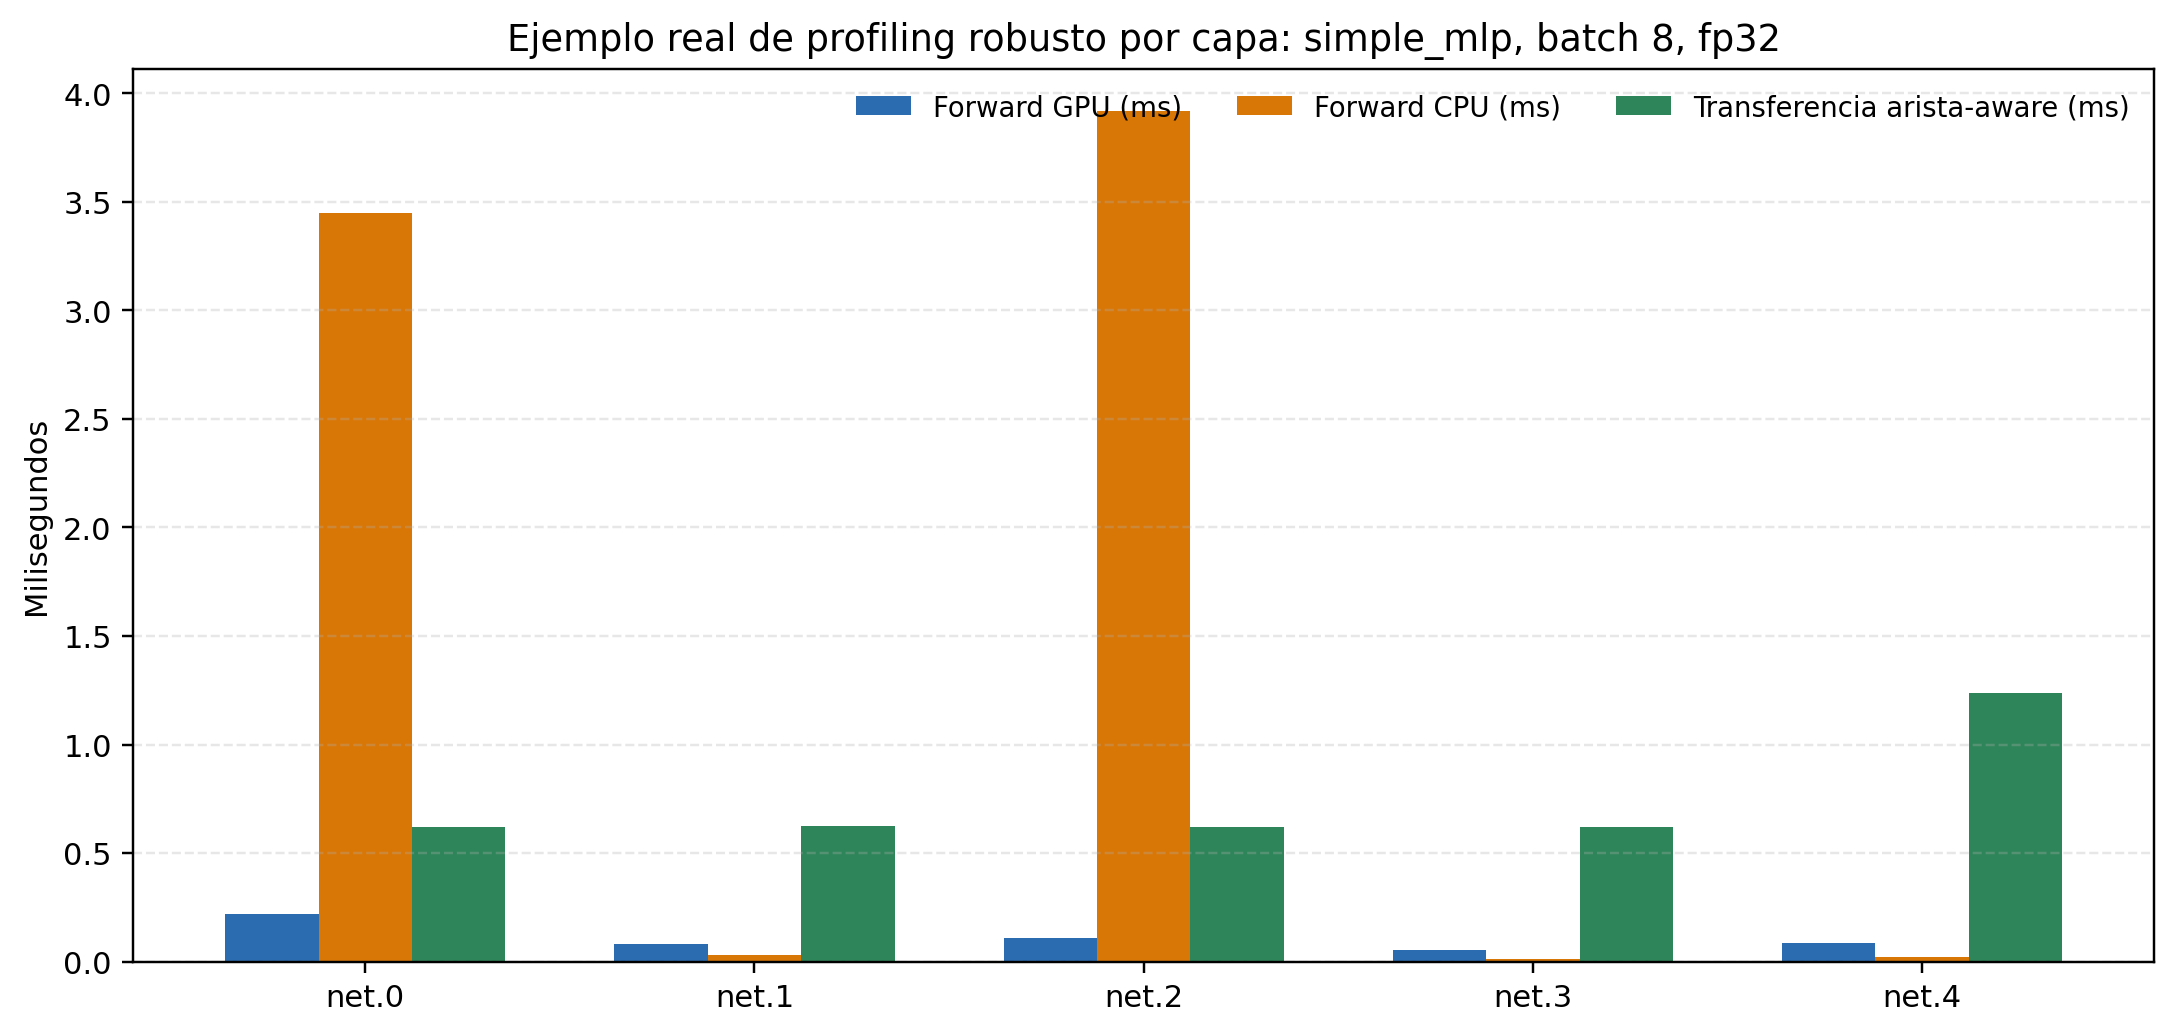
\includegraphics[width=0.95\textwidth]{../reports/thesis_figures/profiling_simple_mlp_layer_costs.png}
\caption{Perfil empirico real por capa para \code{simple_mlp} en smoke con batch 8 y precision \code{fp32}. La figura se genera directamente a partir de \code{simple_mlp_metrics_stats.csv}.}
\label{fig:profiling-layer-costs}
\end{figure}

\begin{table}[t]
\centering
\caption{Contrato minimo de artefactos del pipeline de profiling.}
\label{tab:profiling-artifacts}
\small
\begin{tabularx}{\textwidth}{l l X}
\toprule
Artefacto & Nivel & Rol metodologico \\
\midrule
\code{*_metrics.csv} & capa-corrida & Medicion cruda multicanal \\
\code{*_meta.json} & corrida & Contexto de hardware y politicas \\
\code{*_graph_nodes.csv} & estructura & Nodos con huellas de computo \\
\code{*_graph_edges.csv} & estructura & Dependencias y topologia util \\
\code{*_transfer_edges.csv} & arista & Costos calibrados de comunicacion \\
\code{*_metrics_stats.csv} & agregado & Coeficientes robustos para ILP \\
\bottomrule
\end{tabularx}
\normalsize
\end{table}

\begin{table}[t]
\centering
\caption{Extracto empirico de coeficientes robustos de profiling para \code{simple_mlp}.}
\label{tab:profiling-example-simple-mlp}
\scriptsize
\resizebox{0.92\textwidth}{!}{%
\begin{tabular}{lrrrrl}
\toprule
Capa & GPU fwd (ms) & CPU fwd (ms) & Transferencia (ms) & Memoria GPU (MB) & Calidad \\
\midrule
\code{net.0} & 0.220 & 3.448 & 0.622 & 19.335 & alta dispersion \\
\code{net.2} & 0.110 & 3.918 & 0.621 & 19.343 & alta dispersion \\
\code{net.4} & 0.088 & 0.022 & 1.235 & 19.343 & alta dispersion \\
\bottomrule
\end{tabular}
}
\normalsize
\end{table}

La Tabla~\ref{tab:profiling-example-simple-mlp} deja ver otra propiedad relevante: el problema no se reduce a escoger siempre GPU o siempre CPU. Las capas \code{net.0} y \code{net.2} muestran ventaja de tiempo en GPU pero con una penalizacion de transferencia comparable, mientras que \code{net.4} introduce una frontera de salida con costo comunicativo relativamente alto. Esta estructura de compromiso es precisamente la que vuelve razonable el paso desde profiling empirico hacia optimizacion declarativa.

\section{4.9 Del dato observado al coeficiente de decision}
Una contribucion metodologica menos visible, pero crucial, de este capitulo consiste en establecer la transformacion legitima entre observacion cruda y coeficiente de decision. El punto de partida no es una ecuacion cerrada, sino una nube de eventos con ruido, variabilidad de replica y dependencias contextuales. El punto de llegada no es una estadistica descriptiva neutra, sino un parametro que condiciona una decision binaria ejecutable. Entre ambos extremos media una cadena de validacion que incluye limpieza, agregacion, chequeo de dispersion, verificacion de precision y asociacion estructural con el grafo.

Este pasaje importa porque, en ausencia de dicha cadena, la optimizacion posterior quedaria epistemologicamente suspendida: seria imposible determinar si la solucion ILP mejora realmente la politica de asignacion o simplemente explota artefactos de medicion mal controlados. La tesis evita ese riesgo al convertir el profiling en una etapa con semantica inferencial propia. La decision combinatoria deja de apoyarse en numeros meramente disponibles y pasa a sostenerse en numeros metodologicamente justificados. La diferencia entre medicion disponible y coeficiente defendible es, de hecho, una de las lecciones que separa un benchmark utilitario de un pipeline de decision comparable con propuestas de colocacion automatica de mayor ambicion metodologica \cite{mirhoseini2017device,jia2019beyond}.

\begin{table}[t]
\centering
\caption{Cadena de transformacion desde observacion cruda hasta coeficiente util para optimizacion.}
\label{tab:profiling-inference-chain}
\small
\begin{tabularx}{\textwidth}{lX}
\toprule
Etapa & Funcion inferencial \\
\midrule
Medicion cruda por replica & Captura eventos, tiempos, energia y memoria bajo una configuracion concreta y versionable. \\
Control de validez & Verifica precision efectiva, soporte de hardware, semillas y consistencia basica de ejecucion. \\
Agregacion robusta & Resume tendencia central y dispersion sin colapsar la heterogeneidad experimental relevante. \\
Asociacion estructural & Vincula cada metrica con nodos y aristas del grafo computacional admisible. \\
Coeficiente para ILP & Entrega un escalar interpretable y trazable que puede entrar en funcion objetivo o restricciones. \\
\bottomrule
\end{tabularx}
\normalsize
\end{table}

\notaPendiente{Para la version de deposito conviene anadir aun dos figuras complementarias: la calibracion completa del modelo alpha-beta y una distribucion de replicas por canal para la campana multiservidor.}

\chapter{Formulacion ILP Robusta para Particion Heterogenea CPU-GPU}

\section{5.1 Introduccion y alcance del modelo (congelado en Fase 0)}
La formulacion ILP presentada en este capitulo transforma en decision combinatoria la evidencia empirica construida en el Capitulo 4. El problema no se define sobre costos ideales, sino sobre coeficientes medidos, robustificados y sometidos a criterios de admisibilidad metodologica. Por ello, la principal virtud del modelo no es solo su correccion algebraica, sino la continuidad que preserva entre fenomenologia de runtime y politica ejecutable. Esta continuidad marca una diferencia importante frente a lineas de trabajo donde la colocacion se aprende o se heuristiza sin un contrato tan estricto entre medicion, formulacion y validacion \cite{mirhoseini2017device,jia2019beyond,zheng2022alpa}.

En coherencia con el cierre de Fase 0, el alcance del modelo debe leerse desde la formulacion fuerte comprometida por la tesis: soporte para separacion forward/backward, persistencia de activaciones y compatibilidad con scheduling asincrono. Las ecuaciones base descritas aqui fijan el nucleo de asignacion binaria y costo de corte; las extensiones posteriores muestran como ese nucleo se integra dentro de un sistema mas amplio sin perder interpretabilidad.

\section{5.2 Notacion formal}
Sea $G=(V,E)$ un grafo dirigido aciclico donde cada nodo representa una unidad de computo asignable y cada arista representa una dependencia tensorial potencialmente costosa si se corta entre dispositivos. Para cada nodo se dispone de costos robustos de tiempo, energia y memoria en CPU y GPU; para cada arista se dispone de un costo de transferencia derivado del pipeline de profiling. Esta notacion no surge de una convencion abstracta, sino del contrato de artefactos que enlaza \code{*_metrics_stats.csv}, \code{*_graph_edges.csv} y \code{*_transfer_edges.csv} con el constructor de la instancia ILP.

La ventaja de fijar desde el principio esta correspondencia entre simbolos y artefactos es metodologica. Permite que cada termino del modelo posea una interpretacion operacional y una ruta de verificacion directa en el repositorio. En otras palabras, la notacion formal no reemplaza la trazabilidad; la organiza.

De forma mas explicita, para cada nodo $v \in V$ se consideran coeficientes robustos $T^{gpu}_v$, $T^{cpu}_v$ para tiempo, $E^{gpu}_v$, $E^{cpu}_v$ para energia y $M^{gpu}_v$, $M^{cpu}_v$ para memoria. Para cada arista $(u,v) \in E$ se define un costo de corte $C^{tr}_{uv}$ que resume latencia y volumen de transferencia bajo la calibracion disponible. Adicionalmente, se introducen presupuestos $B_{gpu}$ y $B_{cpu}$ y, en la version extendida del modelo, familias de variables auxiliares para persistencia, recomputacion y decisiones desacopladas de forward y backward. Esta explicitacion conviene porque aclara que el ILP no opera sobre magnitudes abstractas, sino sobre un conjunto de observables transformados en coeficientes de decision.

\section{5.3 Variables de decision}
La variable binaria de asignacion $x_v$ expresa si un nodo se ejecuta en GPU o en CPU, mientras que la variable $y_{uv}$ indica si la arista $(u,v)$ constituye un corte inter-dispositivo. Esta pareja de variables sintetiza la intuicion fisica del problema: toda ganancia local por llevar una capa a GPU puede quedar anulada si dicha decision fragmenta en exceso el grafo e induce comunicacion recurrente.

La inclusion explicita de variables de corte cumple ademas una funcion explicativa en la tesis. Permite descomponer el objetivo total en costo nodal y costo comunicativo, y con ello discutir causalmente por que una solucion supera o no a un baseline greedy. Sin esa explicitud, la optimizacion correria el riesgo de convertirse en una caja negra de asignaciones binarias poco interpretables.

\section{5.4 Funcion objetivo multicriterio}
La funcion objetivo escalariza tiempo, energia y transferencia mediante pesos $w_t$, $w_e$ y $w_{tr}$. La eleccion de esta forma lineal responde a una razon practica y a una razon epistemica. La practica es que mantiene el problema dentro de una clase de resolucion madura y bien entendida. La epistemica es que obliga a declarar con claridad la politica experimental: todo resultado reportado en este capitulo depende de una ponderacion explicita y, por tanto, debe interpretarse como respuesta condicionada a un regimen de preferencias metodologicamente documentado.

Esta escalarizacion no pretende negar la naturaleza multicriterio del problema, sino ofrecer un mecanismo auditable para recorrer regiones del espacio de compromiso. Los barridos sobre presupuestos GPU y los estudios de sensibilidad posteriores cumplen precisamente la funcion de mostrar hasta que punto la solucion cambia cuando cambian los pesos o la factibilidad fisica.

En su forma base, la funcion objetivo puede escribirse como

$$
\min Z = w_t \sum_{v \in V}\left[x_v T^{gpu}_v + (1-x_v)T^{cpu}_v\right]
	+ w_e \sum_{v \in V}\left[x_v E^{gpu}_v + (1-x_v)E^{cpu}_v\right]
	+ w_{tr} \sum_{(u,v) \in E} y_{uv} C^{tr}_{uv}.
$$

Esta expresion deja ver una hipotesis central del modelo: el costo total se descompone en contribuciones nodales y contribuciones de corte. La linealidad no afirma que el hardware sea realmente lineal en todos sus efectos, sino que la aproximacion adoptada es suficientemente interpretable y operativa para sostener una politica de decision auditable. La tesis asume esa simplificacion de forma explicita para poder discutir luego, con rigor, donde estan sus limites y que fenomenos quedan fuera de la envolvente del modelo.

\section{5.5 Linealizaciones exactas y restricciones}
La linealizacion exacta de la variable de corte mediante desigualdades sobre $x_u$, $x_v$ e $y_{uv}$ preserva fidelidad semantica sin abandonar el dominio MILP. Esto es importante porque evita recurrir a aproximaciones que podrian abaratar artificialmente ciertos cortes o alterar la logica del problema. Las restricciones de memoria por dispositivo, por su parte, convierten la solucion en una politica fisicamente viable y no solo en una mejora aritmetica sobre papel.

Desde el punto de vista de tesis, la relevancia de estas restricciones va mas alla de su contenido tecnico. Cada una representa una salvaguarda contra conclusiones vacias: sin linealizacion correcta no hay semantica fiable del corte; sin presupuestos de memoria no hay viabilidad operativa; sin dominio binario no hay puente directo hacia el runtime.

Una formulacion minima de estas condiciones puede expresarse como

$$
y_{uv} \ge x_u - x_v, \qquad
y_{uv} \ge x_v - x_u,
$$

acompanada por

$$
y_{uv} \le x_u + x_v, \qquad
y_{uv} \le 2 - (x_u + x_v),
$$

de modo que $y_{uv}$ capture exactamente la discrepancia binaria entre extremos de la arista. A ello se anaden restricciones de memoria del tipo

$$
\sum_{v \in V} x_v M^{gpu}_v \le B_{gpu}, \qquad
\sum_{v \in V} (1-x_v) M^{cpu}_v \le B_{cpu},
$$

que convierten la factibilidad en una condicion estructural del problema. En la version extendida, estas desigualdades se enriquecen con variables asociadas a retencion y recomputacion, pero la idea permanece: la solucion debe ser simultaneamente interpretable, resoluble y ejecutable.

\section{5.6 Robustificacion estadistica}
La robustificacion mediante $\mu + k_\sigma\sigma$ expresa de forma compacta una decision metodologica profunda: las politicas de particion no deben optimizar solo el promedio, sino una version del costo que incorpora incertidumbre observada. Este desplazamiento es especialmente valioso en infraestructura heterogenea, donde el ruido por replica, la variabilidad termica o los efectos de scheduler pueden volver fragil una solucion ajustada al promedio puntual. En terminos conceptuales, la eleccion se emparenta con la intuicion que subyace a los esquemas clasicos de checkpointing y reduccion de memoria: no basta con un costo esperado atractivo si la politica resultante se apoya en un regimen experimental inestable \cite{griewank2000revolve,chen2016sublinear}.

En el proyecto, el parametro $k_\sigma$ se ha estudiado con barridos controlados. Sobre el caso smoke de \code{simple_mlp}, el valor base $k_\sigma=1.0$ produce un objetivo ILP de 1.810442 a 64 MB de presupuesto GPU; reducirlo a 0.0 genera una solucion mas optimista con objetivo 1.310637, mientras incrementarlo a 2.0 eleva el objetivo a 2.310246. Este comportamiento confirma que $k_\sigma$ opera efectivamente como un mando de conservadurismo controlado.

La interpretacion de esta robustificacion debe explicitarse con cuidado. El modelo no pretende construir una teoria probabilistica completa de la incertidumbre, sino introducir una proteccion operacional contra soluciones demasiado sensibles al promedio puntual. En ese sentido, $k_\sigma$ funciona como un parametro de aversion al riesgo experimental: cuanto mayor es su valor, mayor es la penalizacion que la formulacion impone a coeficientes observados con alta dispersion. La tesis considera esta operacion como una decision metodologica defendible porque traslada al modelo una propiedad real del dato: su estabilidad observacional.

\section{5.7 Integracion multi-hardware}
Cuando se dispone de perfiles equivalentes provenientes de varios hosts, la tesis propone dos politicas de fusion: peor caso por coeficiente y media mas dispersion inter-host. La primera prioriza seguridad operacional; la segunda busca equilibrio entre rendimiento promedio y heterogeneidad del parque. En ambos casos, la agregacion multi-hardware se concibe como un mecanismo de transferibilidad, no como una etapa cosmetica de posprocesado.

Este punto es central para el cierre doctoral pendiente. El repositorio ya contiene runbooks y protocolo metodologico para construir el dataset multi-servidor; lo que falta es ejecutar esa campaña con suficiencia estadistica. Por tanto, la integracion multi-hardware debe presentarse en este borrador como capacidad ya dispuesta metodologicamente, pero aun en proceso de consolidacion empirica plena.

\section{5.8 Complejidad y trazabilidad}
Si el grafo tiene $n$ nodos y $m$ aristas, el modelo introduce $n+m$ variables binarias y un numero de restricciones dominado por las linealizaciones de corte. Esta observacion importa porque delimita la escalabilidad practica del enfoque y justifica la existencia de backends diferenciados: `pulp` con CBC para resolucion general, `exhaustive` para subinstancias pequenas usadas como oraculo metodologico y `auto` para seleccion pragmatica de backend.

La trazabilidad del solver se refuerza mediante artefactos de salida estructurados, entre ellos \code{ilp_assignment.csv}, \code{ilp_cut_edges.csv} e \code{ilp_solution_summary.json}. Esta tripleta permite auditar la solucion desde tres perspectivas: politica por nodo, cortes inducidos y resumen global de factibilidad y objetivo. En una tesis aplicada, tal descomposicion reduce la distancia entre ecuacion y resultado observable.

Conviene anadir que la complejidad computacional del problema no se invoca aqui como argumento de autoridad, sino como limite practico que orienta el diseno experimental. Saber que la formulacion crece con el numero de nodos y aristas permite entender por que el manuscrito combina diferentes backends y por que algunas campañas se ejecutan en regimen smoke o controlado antes de ampliarse. La tesis no oculta esta restriccion; la incorpora como parte de la honestidad metodologica del modelo.

\section{5.9 Supuestos de modelado y frontera de aplicabilidad}
Todo modelo declarativo fuerte descansa sobre supuestos que deben hacerse visibles. En esta tesis destacan al menos cinco. Primero, se asume que el grafo disponible conserva suficiente fidelidad estructural para que los cortes tengan significado fisico. Segundo, se asume que los coeficientes robustificados son una aproximacion razonable del costo efectivo por nodo y por arista bajo el regimen experimental considerado. Tercero, se asume que la escalarizacion lineal es adecuada para explorar compromisos entre tiempo, energia y transferencia sin ocultar por completo su semantica. Cuarto, se asume que las restricciones de memoria sintetizan de manera util el principal cuello de botella de factibilidad. Quinto, se asume que el paso desde solucion a plan puede preservarse sin redefinir silenciosamente la politica entre optimizacion, simulacion y runtime.

Ninguno de estos supuestos es inocente. Cada uno fija una frontera de aplicabilidad del modelo y, por tanto, un limite de generalizacion de sus resultados. La fuerza del manuscrito no consiste en negar esa dependencia, sino en explicitarla y someterla a validacion cruzada por sensibilidad, ablacion y contraste operacional. Ese es precisamente el rasgo que distingue una formulacion doctoral de una heuristica utilitaria: no solo produce soluciones, sino que declara bajo que hipotesis esas soluciones deben tomarse en serio.

\section{5.10 Validacion comparativa contra baselines (habilitada por Fase 1)}
La validacion comparativa frente a baselines cumple una funcion decisiva: distinguir si la mejora procede realmente de la estructura del modelo o de una ventaja trivial facilmente alcanzable sin ILP. En el conjunto smoke consolidado de Fase 1, el mejor punto factible para \code{simple_mlp} a 64 MB muestra un objetivo ILP de 1.810 frente a 27.153 para \code{all_cpu} y 2.035 para \code{greedy}, lo que equivale a una mejora del 93.33\% respecto a \code{all_cpu} y del 11.06\% respecto a \code{greedy}.

Este resultado no debe sobredimensionarse: corresponde a una malla reducida y a un modelo piloto. Sin embargo, si constituye evidencia valida de que la formulacion, incluso en regimen smoke, ya supera tanto a una politica trivial como a una heuristica nodal. Ese hecho justifica la expansion posterior hacia campañas mas amplias y hacia comparativas sobre hardware fusionado.

\begin{figure}[t]
\centering
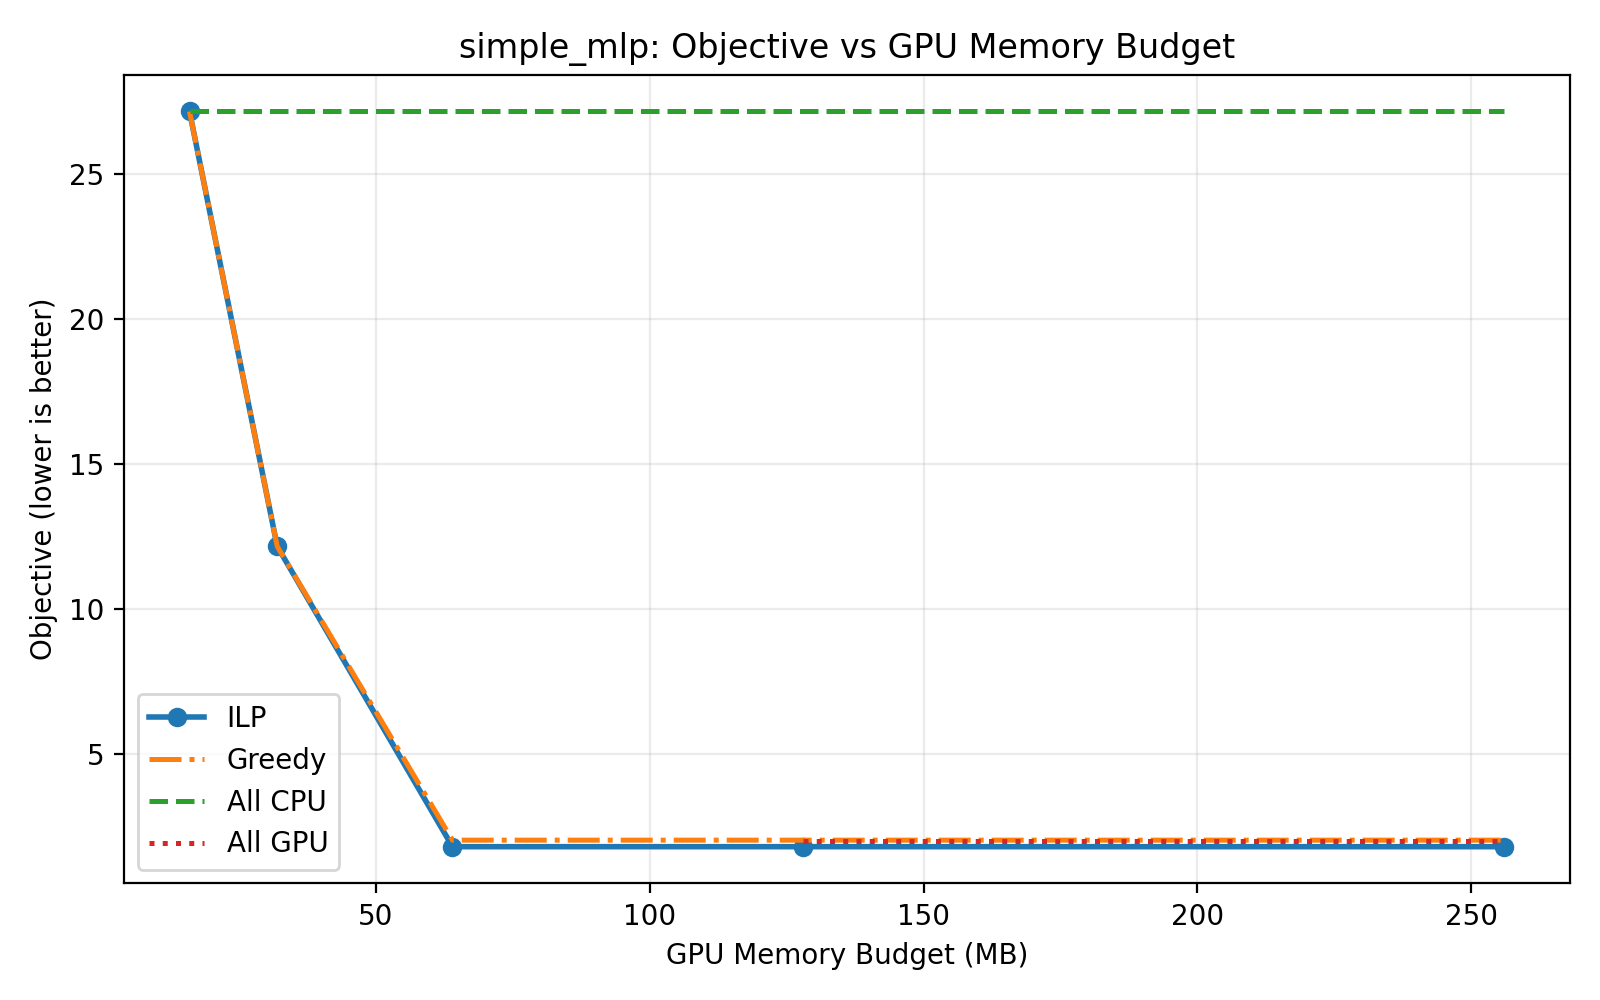
\includegraphics[width=0.78\textwidth]{../reports/ilp_results_phase1_smoke/simple_mlp_objective_vs_budget.png}
\caption{Frontera de compromiso objetivo-presupuesto GPU para el caso smoke consolidado de \code{simple_mlp}.}
\label{fig:ilp-budget-smoke}
\end{figure}

\begin{table}[t]
\centering
\caption{Mejor resultado ILP factible por modelo bajo los presupuestos GPU evaluados en el conjunto smoke.}
\label{tab:ilp-best-per-model-sanitized}
\scriptsize
\resizebox{\textwidth}{!}{%
\begin{tabular}{lrrrrrrrr}
\toprule
Modelo & Budget GPU & Obj. ILP & Obj. CPU & Obj. Greedy & Mejora vs CPU (\%) & Mejora vs Greedy (\%) & Capas GPU & Cortes \\
\midrule
\code{simple_mlp} & 64 & 1.810 & 27.153 & 2.035 & 93.33 & 11.06 & 3 & 1 \\
\bottomrule
\end{tabular}
}
\normalsize
\end{table}

\section{5.11 Estudios de sensibilidad (habilitados por Fase 1)}
Los estudios de sensibilidad muestran que la formulacion no solo produce una solucion puntual, sino una respuesta interpretable ante perturbaciones controladas de sus parametros. En el conjunto smoke, el barrido sobre $k_\sigma$ exhibe una variacion aproximadamente lineal del objetivo en torno al punto base, mientras que el barrido sobre $w_{transfer}$ revela un comportamiento monotono pero no lineal: cuando $w_{transfer}=0.0$, el modelo tolera tres cortes y reordena capas hacia una solucion mas agresiva; al aumentar el peso de transferencia, la politica reduce fragmentacion y encarece el objetivo total bajo una lectura mas conservadora del sistema.

Esta informacion es de interes doctoral porque permite afirmar que los parametros del modelo tienen semantica economica verificable. No son perillas arbitrarias, sino mecanismos de politica cuyo efecto sobre la solucion puede estudiarse con trazas reproducibles.

\section{5.12 Ablaciones formales (habilitadas por Fase 1)}
La suite de ablaciones cumple la funcion de desagregar el aporte de los componentes metodologicos del modelo. En el resumen disponible para \code{simple_mlp}, la variante completa obtiene objetivo 1.810442; eliminar la robustificacion reduce el objetivo en 0.499805 unidades, reflejando un escenario optimista irreal; eliminar topologia o costos de transferencia reduce el objetivo en 0.438429 unidades y altera la estructura de la particion, pasando de un plan con un corte y tres capas en GPU a variantes mas fragmentadas o semantica empobrecida.

Estas ablaciones son importantes porque muestran que la mejora no proviene solo de un solver aplicado sobre cualquier costo disponible. Proviene de la conjuncion entre grafo admisible, penalizacion comunicativa y robustificacion estadistica. En ausencia de alguno de esos componentes, el problema resuelto cambia de significado.

\begin{table}[t]
\centering
\caption{Barrido Pareto ILP en el conjunto smoke con comparacion frente a baselines.}
\label{tab:ilp-budget-sweep-sanitized}
\scriptsize
\resizebox{0.92\textwidth}{!}{%
\begin{tabular}{rrrrrrr}
\toprule
Budget GPU & Obj. ILP & Obj. Greedy & Obj. CPU & Mejora vs CPU (\%) & Mejora vs Greedy (\%) & Cortes \\
\midrule
16 & 27.153 & 27.153 & 27.153 & 0.00 & 0.00 & 0 \\
32 & 12.163 & 12.163 & 27.153 & 55.20 & 0.00 & 1 \\
64 & 1.810 & 2.035 & 27.153 & 93.33 & 11.06 & 1 \\
128 & 1.810 & 2.035 & 27.153 & 93.33 & 11.06 & 1 \\
256 & 1.810 & 2.035 & 27.153 & 93.33 & 11.06 & 1 \\
\bottomrule
\end{tabular}
}
\normalsize
\end{table}

\section{5.13 Extension avanzada: persistencia de activaciones y rematerializacion (Fase 4)}
La extension avanzada deja de ser prospectiva en el estado actual del proyecto. La Fase 4 ha integrado decision dual forward/backward, persistencia de activaciones, recomputacion, checkpointing y compatibilidad con prefetching en \code{src/ilp/advanced_terms.py}, \code{src/ilp/model_builder.py} y en el runtime asociado. Esto permite afirmar que la tesis no se cierra sobre un ILP minimamente viable, sino sobre una version extendida cuyo significado operacional ya fue contrastado en evidencia controlada. La articulacion entre persistencia, recomputacion y particion heterogenea enlaza directamente con la tradicion inaugurada por Revolve y retomada despues por estrategias de memoria sublineal y offloading, aunque aqui se reinterpreta como decision conjunta dentro de una formulacion declarativa unificada \cite{griewank2000revolve,chen2016sublinear,ren2021zerooffload}.

No obstante, desde el punto de vista de escritura doctoral conviene mantener una distincion clara entre dos niveles de evidencia. Existe ya evidencia operacional de que la extension funciona y puede ejecutarse sobre un caso dual controlado; lo que aun falta es una explotacion experimental amplia de esa extension sobre una matriz final de modelos y hosts. El manuscrito debe sostener ambas verdades sin confundir madurez de implementacion con amplitud de validacion empirica.

\section{5.14 Amenazas a la validez}
Las amenazas a la validez del modelo ILP se agrupan en tres clases. La primera es la amenaza de medicion: coeficientes sesgados por ruido, precision degradada o muestra insuficiente pueden inducir optimizaciones sobre un problema mal especificado. La segunda es la amenaza de modelado: la linealidad no captura todas las interacciones no lineales del hardware, como saturacion de bus o contencion compartida. La tercera es la amenaza de transferibilidad: una politica afinada sobre un host unico puede no generalizar a un parque heterogeneo.

Las mitigaciones ya integradas en el proyecto son sustantivas: compuertas de admisibilidad sobre calidad muestral y procedencia estructural, barridos de sensibilidad, ablaciones, comparacion con baselines y capacidad de fusion multi-hardware. Aun asi, el cierre doctoral pleno exige ejecutar el protocolo multi-servidor y ampliar la base de evidencia sobre calidad final del entrenamiento. La necesidad de este cierre adicional no contradice la validez del modelo; la situa, con honestidad, en el mismo horizonte comparativo en el que la literatura reciente ha tenido que conciliar capacidad de optimizacion con diversidad real de plataformas \cite{rajbhandari2020zero,ren2021zerooffload,zheng2022alpa}.

Visto desde una perspectiva mas amplia, este capitulo cumple una funcion que trasciende la simple obtencion de una solucion optima. Su papel es mostrar que la asignacion heterogenea puede formularse como decision cientificamente discutible, y no solo como una heuristica afortunada. El ILP obliga a explicitar hipotesis de costo, restricciones fisicas y relaciones entre nodos y cortes. Esa explicitud es una ganancia epistemologica en si misma, porque permite que el lector cuestione y refine el modelo sin perder de vista que toda modificacion tiene consecuencias operacionales precisas.

\begin{table}[t]
\centering
\caption{Amenazas a la validez del modelo ILP y estado de mitigacion.}
\label{tab:ilp-validity-threats}
\scriptsize
\setlength{\tabcolsep}{4pt}
\begin{tabularx}{\textwidth}{lXX}
\toprule
Amenaza & Mitigacion ya integrada & Evidencia pendiente de cierre \\
\midrule
Medicion sesgada o inestable & Profiling con replicas, robustificacion estadistica, control de precision efectiva y banderas de calidad & Campana multiservidor con base estadistica ampliada \\
Modelo lineal insuficiente & Sensibilidad, ablaciones y contraste posterior con simulacion y runtime & Calibraciones no lineales y estudios de saturacion a mayor escala \\
Falta de transferibilidad entre hosts & Diseno metodologico para fusion multi-hardware y protocolo de validacion transversal & Consolidacion empirica del dataset inter-host y su explotacion final \\
Brecha entre solver y ejecucion real & Representacion formal de plan, simulador y runtime con trazabilidad de procedencia & Matriz mas amplia de contraste prediccion-observacion \\
\bottomrule
\end{tabularx}
\normalsize
\end{table}

La Tabla~\ref{tab:ilp-validity-threats} deja ver que las amenazas a la validez no son un apartado defensivo secundario, sino una parte constitutiva del sentido doctoral del capitulo. Explicitar que esta mitigado, que permanece abierto y bajo que protocolo se resolvera es una forma de honestidad cientifica, pero tambien una forma de fortalecer la interpretabilidad de la solucion obtenida.

\chapter{Ejecucion Hibrida, Simulacion y Validacion Experimental}

\section{6.1 Introduccion: cierre del bucle planificacion-ejecucion}
Se formaliza la transicion desde solucion de optimizacion hacia comportamiento operacional verificable.

\section{6.2 Representacion formal del plan de ejecucion (Fase 2)}
Se define la estructura de plan, sus invariantes y su semantica de consumo por componentes runtime.

\section{6.3 Simulador hibrido: arquitectura y validacion topologica (Fase 2)}
Se describe el diseno del simulador y los chequeos de coherencia sobre el DAG de ejecucion.

\section{6.4 Estudio de prediccion: latencia, memoria y costos de transferencia (Fase 2)}
Se especifican metricas de prediccion y metodologia para evaluacion determinista previa a ejecucion real.

\section{6.5 Implementacion del ejecutor hibrido en PyTorch (Fase 3)}
Se documentara la implementacion operacional de la politica de asignacion en entrenamiento real.

\section{6.6 Baselines reales y comparativos experimentales (Fase 3)}
Se establecera comparacion sistematica frente a politicas de referencia en entorno fisico.

\section{6.7 Prediccion frente a observacion: contraste operacional (Fase 3)}
Se cuantificara el error de prediccion y su distribucion por regimen de carga.

\section{6.8 Exactitud final del modelo y estabilidad de convergencia (Fase 3-5)}
Se evaluara impacto de la ejecucion hibrida sobre calidad final del entrenamiento.

\section{6.9 Extensiones con persistencia de activaciones y scheduling asincrono (Fase 4)}
Se integraran extensiones avanzadas de memoria y planificacion para cerrar la propuesta completa.

\section{6.10 Analisis integrado de resultados y limites experimentales (Fase 5)}
Se sintetizaran resultados globales y restricciones metodologicas observadas en campana doctoral.

\chapter{Conclusiones, Limites y Trabajo Futuro}

\section{7.1 Sintesis de resultados frente a la hipotesis}
La hipotesis central de la tesis afirma que una politica de particion heterogenea CPU-GPU, construida a partir de evidencia empirica robusta y optimizacion declarativa, puede mejorar el comportamiento global frente a politicas simples sin perder validez operacional. A la fecha de este borrador, esa hipotesis ya cuenta con sustento parcial fuerte. El pipeline de profiling existe y produce coeficientes admisibles; el ILP supera a baselines \code{all_cpu} y \code{greedy} en el caso smoke consolidado; la solucion puede transformarse en plan, simularse y ejecutarse en runtime; y la version extendida con decisiones duales y prefetching ya ha sido materializada en evidencia controlada.

El resultado mas claro disponible en esta etapa es el cierre del circuito metodologico minimo. La tesis ya puede afirmar que mide, decide, simula y ejecuta. Lo que aun no puede afirmar con igual amplitud es la universalidad de ese comportamiento sobre una matriz multi-servidor y multi-arquitectura estadisticamente amplia. Por ello, la hipotesis debe presentarse en este borrador como fuertemente apoyada en viabilidad metodologica y en evidencia focal, pero pendiente de cierre empirico transversal final.

\section{7.2 Contribuciones metodologicas y de sistemas}
Las contribuciones del trabajo pueden sintetizarse en cuatro niveles complementarios. Primero, se construye un sistema de profiling por capa que integra tiempo, energia, memoria, transferencia y procedencia estructural del grafo bajo un contrato de artefactos reproducible. Segundo, se formula un ILP robusto e interpretable que traduce esa evidencia en una decision binaria ejecutable bajo restricciones de memoria y con soporte para sensibilidad, ablaciones y fusion multi-hardware. Tercero, se cierra el puente entre optimizacion y sistemas mediante una representacion formal del plan, un simulador determinista y un ejecutor hibrido observacional. Cuarto, se fija un contrato metodologico que obliga a sostener cada afirmacion con evidencia trazable y que distingue explicitamente entre capacidad implementada, validacion focal y cierre doctoral amplio.

La contribucion original del proyecto no reside solamente en cada pieza aislada, sino en su integracion rigurosa. Ese caracter de sistema completo es el que diferencia esta tesis de propuestas que permanecen en el plano del benchmarking, del modelado offline o del prototipo runtime sin trazabilidad suficiente.

\begin{figure}[t]
\centering
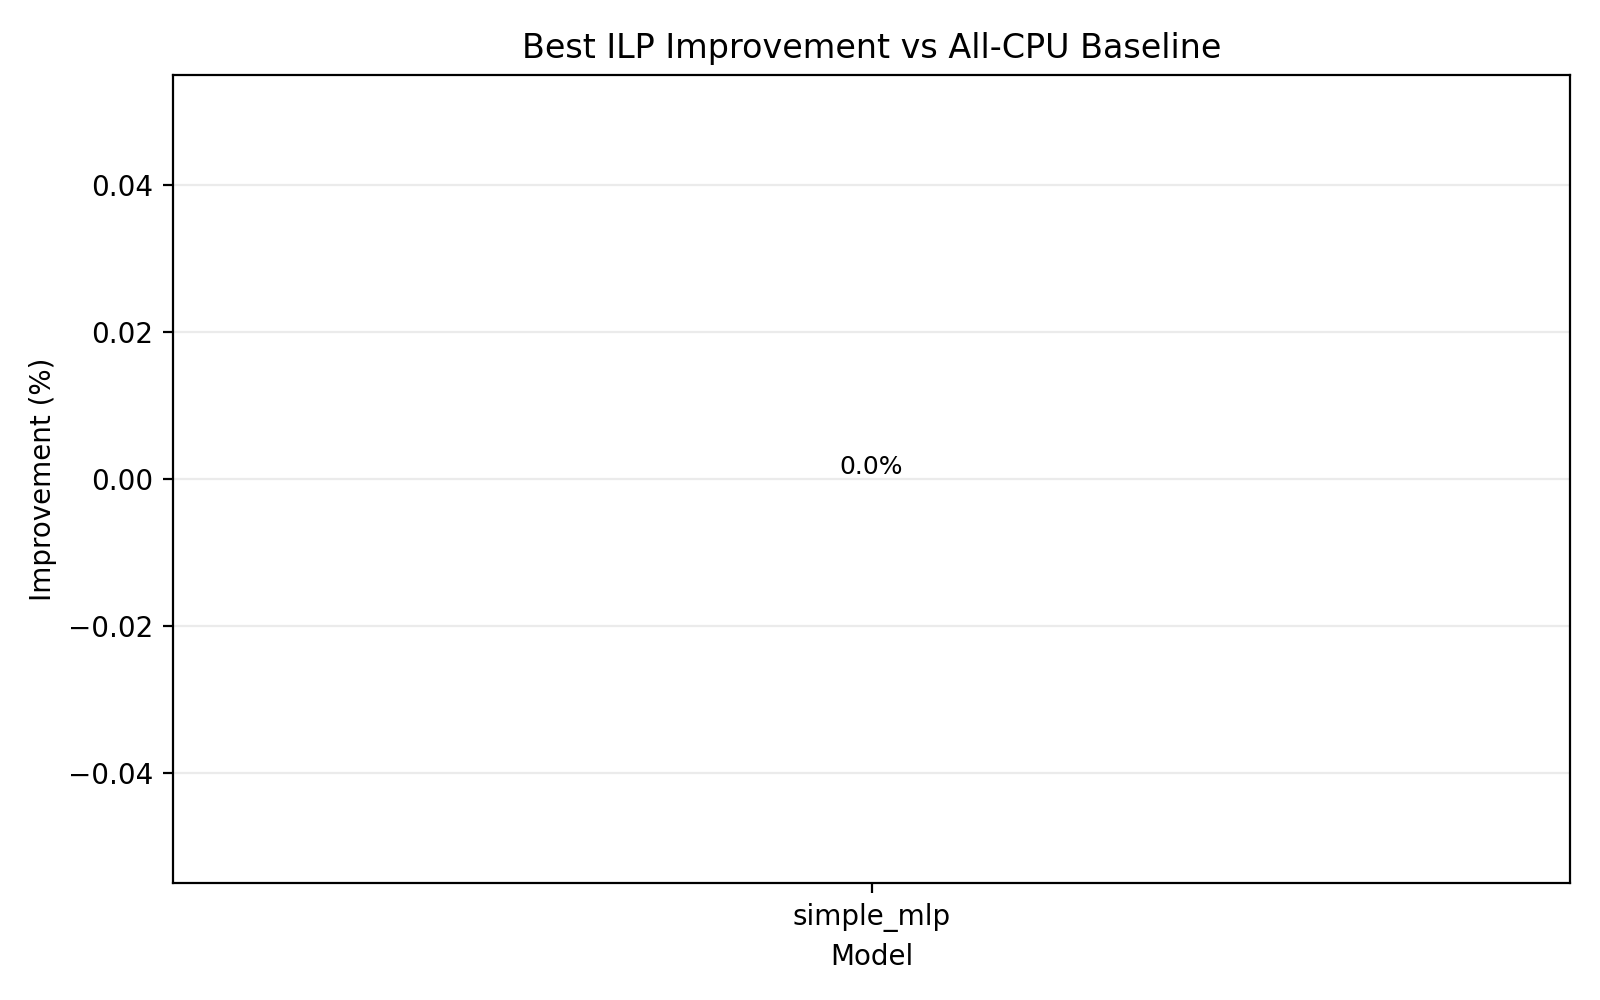
\includegraphics[width=0.82\textwidth]{../reports/ilp_results_phase1/best_ilp_vs_all_cpu_improvement.png}
\caption{Mejora porcentual del mejor plan ILP frente al baseline \code{all_cpu} en la campana de Fase 1. Esta figura resume la direccion favorable de la evidencia ILP antes del cierre empirico multi-servidor.}
\label{fig:ilp-vs-all-cpu}
\end{figure}

\section{7.3 Limites del modelo y del protocolo experimental}
El trabajo presenta limites que deben exponerse con precision. En el plano de modelado, la formulacion lineal no capta todas las no linealidades del hardware real, y el modelo alpha-beta de transferencia sigue siendo una aproximacion de primer orden. En el plano empirico, parte de la evidencia disponible procede todavia de mallas smoke o de casos controlados sobre modelos piloto, lo que restringe la generalizacion inmediata de ciertas conclusiones. En el plano experimental, la principal limitacion abierta es la ausencia de una campaña multi-servidor final completamente cerrada con al menos cinco replicas por configuracion en la malla canonica.

Existe ademas un limite narrativo que la tesis debe evitar: confundir madurez del software con amplitud de la validacion. El repositorio ya incorpora capacidades avanzadas como separacion forward/backward, persistencia de activaciones y prefetching; sin embargo, su explotacion estadistica amplia aun esta en curso. La conclusion correcta, por tanto, no es que el sistema este incompleto, sino que su cierre empirico de nivel doctoral todavia requiere una campaña final mas extensa.

\section{7.4 Lineas de trabajo futuro}
Las lineas de trabajo futuro se desprenden con claridad del estado actual del proyecto. La primera y mas inmediata es ejecutar la validacion multi-servidor definida en el protocolo metodologico del repositorio, consolidando un dataset heterogeneo que permita resolver ILP robusto inter-host y contrastar su transferibilidad real. La segunda es cerrar la comparacion sistematica prediccion-versus-observacion sobre una matriz final de modelos, no solo sobre casos piloto. La tercera es profundizar en la validacion de calidad final del entrenamiento, integrando accuracy, loss o metrica especifica de tarea como condicion de aceptacion tan relevante como tiempo o memoria.

Una cuarta linea, mas propiamente investigativa, consiste en enriquecer el modelo de costo con terminos no lineales o calibraciones por tramos que capturen saturacion y contencion de bus con mayor fidelidad. Una quinta es ampliar el estudio a familias de modelos mas grandes y a regimens de precision mas diversos, siempre que se preserve el mismo contrato de trazabilidad y admisibilidad metodologica. Estas extensiones no invalidan el nucleo actual del trabajo; lo prolongan hacia una agenda de investigacion posterior coherente con los limites ya identificados.

\section{7.5 Trazabilidad final entre afirmaciones y evidencia}
Una monografia doctoral sobre sistemas no se cierra adecuadamente solo con una enumeracion de aportes; debe explicitar la correspondencia entre cada afirmacion fuerte y la evidencia que la sostiene. La tabla siguiente resume esa relacion y fija, de manera deliberadamente conservadora, el alcance con el que cada resultado puede presentarse en esta etapa del manuscrito.

\begin{table}[t]
\centering
\caption{Trazabilidad entre afirmaciones nucleares del manuscrito y evidencia disponible.}
\label{tab:thesis-traceability}
\scriptsize
\setlength{\tabcolsep}{4pt}
\begin{tabularx}{\textwidth}{p{0.26\textwidth}X p{0.19\textwidth}}
\toprule
Afirmacion & Evidencia principal en el manuscrito & Alcance actual \\
\midrule
El proyecto produce coeficientes empiricos trazables por capa & Capitulo 4, Tabla~\ref{tab:profiling-artifacts}, Figura~\ref{fig:profiling-layer-costs}, Tabla~\ref{tab:profiling-example-simple-mlp} & Demostrado \\
La formulacion ILP supera baselines simples en casos consolidados & Capitulo 5, Figura de objetivo vs presupuesto y tablas de comparacion ILP & Demostrado en campanas focales \\
La solucion ILP puede transformarse en plan, simularse y ejecutarse & Capitulo 6, secciones de representacion, simulacion y ejecutor hibrido & Demostrado \\
Existe contraste predictivo en un caso controlado & Capitulo 6, Figura~\ref{fig:prediction-vs-observation} y Tabla~\ref{tab:prediction-vs-observation} & Demostrado en caso focal \\
Las extensiones duales y de prefetching tienen evidencia operacional & Capitulo 6, evidencia controlada de Fase 4 y discusion de extensiones avanzadas & Demostrado en validacion controlada \\
La tesis ya dispone de cierre empirico transversal multi-servidor & Protocolo multiservidor y discusion de limites en Capitulos 6 y 7 & Pendiente \\
\bottomrule
\end{tabularx}
\normalsize
\end{table}

La funcion de esta tabla no es solo resumir resultados, sino disciplinar la escritura final. Obliga a distinguir entre lo ya demostrado, lo demostrado solo en regimen focal y lo que aun debe completarse antes del deposito definitivo. Esa distincion es parte de la calidad epistemologica del manuscrito y protege la tesis frente a sobreafirmaciones.

\section{7.6 Valor doctoral del trabajo en su estado actual}
El valor doctoral del manuscrito, en su estado presente, no debe medirse exclusivamente por la cantidad de funcionalidad implementada ni por la longitud del documento, sino por la coherencia alcanzada entre problema, metodo y evidencia. A este nivel, la tesis ya exhibe un rasgo fuerte: ha transformado una intuicion de ingenieria sobre infrautilizacion de CPU y saturacion de memoria de GPU en una cadena argumental completa que incluye fundamento teorico, observacion empirica, formulacion declarativa, simulacion y validacion operacional. Ese encadenamiento no es trivial y constituye, por si mismo, una contribucion metodologica robusta.

Tambien es importante subrayar que el manuscrito ya se encuentra mas alla del estadio de propuesta conceptual. Existe un pipeline que produce artefactos, un modelo que resuelve decisiones no triviales, una semantica de plan que cierra el paso hacia simulacion y runtime, y evidencia focal de que las extensiones mas ambiciosas del alcance fuerte pueden materializarse de forma controlada. En consecuencia, la tesis no esta en una fase de mera promesa investigativa; se encuentra en una fase de consolidacion y ampliacion empirica. Esa diferencia debe quedar clara porque condiciona el modo en que se presentan tanto los aportes como las limitaciones.

Sin embargo, precisamente por esa madurez, el documento tiene la obligacion de sostener un criterio alto de prudencia interpretativa. Una tesis doctoral rigurosa no solo debe demostrar que puede hacer algo, sino delimitar con claridad donde termina la evidencia efectivamente disponible. El cierre multi-servidor, la ampliacion estadistica de la validacion y la consolidacion final de calidad del entrenamiento no son detalles secundarios: son las piezas que convertiran una demostracion fuerte de viabilidad metodologica en una afirmacion generalizable de alcance doctoral pleno. La honestidad con que el manuscrito marca esa frontera constituye una parte esencial de su calidad cientifica.

\section{7.7 Cierre final}
La pregunta que ha organizado esta investigacion puede formularse de manera simple: es posible redistribuir de forma cientificamente justificada el entrenamiento profundo entre CPU y GPU para aliviar la presion de memoria sin degradar el valor operacional del proceso. La respuesta que el manuscrito ya puede ofrecer es igualmente clara, aunque matizada: si, bajo un regimen metodologico que mida, modele, simule y observe la politica resultante. Esa condicionalidad no debilita la respuesta; la convierte en una tesis verificable y no en una intuicion optimista.

En ultima instancia, la contribucion del trabajo consiste en mostrar que la heterogeneidad computacional puede dejar de ser un trasfondo pasivo del entrenamiento para convertirse en objeto explicito de decision. Esa transformacion conceptual tiene implicaciones que exceden el caso concreto estudiado: invita a pensar el aprendizaje profundo no solo como optimizacion estadistica sobre datos y parametros, sino tambien como organizacion formal de recursos materiales escasos. En esa interseccion entre teoria del entrenamiento, sistemas heterogeneos y metodologia experimental se situa el nucleo intelectual de la monografia.

El cierre definitivo del doctorado exigira, todavia, ampliar y consolidar la evidencia transversal. Pero aun en su forma actual, el manuscrito ya fija una posicion fuerte: la particion heterogenea CPU-GPU no debe abordarse como una coleccion de ajustes aislados, sino como una politica formal, empiricamente calibrada y operacionalmente contrastable. Ese es el sentido profundo del trabajo y el criterio bajo el cual debe leerse su aportacion.


\end{document}
